\documentclass[ a4paper, twocolumn]{article}

\usepackage[utf8]{inputenc}
\usepackage{mathtools}
\usepackage{amsmath}
\usepackage{color}
\usepackage{a4wide}
\usepackage{graphicx}
\usepackage{indentfirst}
\usepackage{url}
\usepackage{listings}
\usepackage{caption}

\lstset{
language=Python,
basicstyle=\small\sffamily,
numbers=left,
numberstyle=\tiny,
xleftmargin = 3em,
frame=tb,
columns=fullflexible,
showstringspaces=false,
}

\title{Análise de Algoritmos}
\author{Vinicius A. Matias}
\date{\today}
\begin{document}
\maketitle

\section{Introdução}
Muitos problemas reais podem ser aplicados computacionalmente por meio de algoritmos. A área de análise de algoritmos visa estudar e projetar algoritmos com base no tempo e espaço ocupado para uma solução ótima (de menor custo possível). 

As maneiras mais comuns para medir o custo de algoritmos são: medição direta (medir o tempo de processamento com base no tempo real, logo, é influenciado pelo hardware); custo baseado em um computador ideal (valores tabulados  por linguagem de programação para medir o custo de cada operação); e por meio das operações mais significativas (mais utilizada, focando em identificar as operações que aumentam o custo do algoritmo).

\section{Função de complexidade}

Para a análise de complexidade seguindo a operação de maior custo, podemos definir uma função de complexidade $f(n)$, onde n é o tamanho da entrada e $f(n)$ é o número de comparações necessárias para resolver um problema. Vamos exemplificar o problema utilziando o trecho de código em Python na Listing 1. Este código recebe um vetor ou lista A, que tem tamanho n (determinado por pelo comando \textit{len()}.

\begin{lstlisting}[label=max_array,caption= Maior valor de um arranjo]
def max_array(A):
    max = A[0]
    i = 1
    
    while i < len(A):
        if A[i] > max:
            max = A[i]  
        i += 1
    
    return max
\end{lstlisting}

A operação crítica para este algoritmo é determinada pelo \textit{if} da linha 6, cuja troca pode ser feita, no pior caso, n-1 vezes. Note que antes de se iniciar o loop, max é definido como o primeiro valor do arranjo, consequentemente, é desnecessário utilizar este valor no while (logo, o loop começa do segundo valor e vai até o último, com n-1 comparações). Portante, a função de complexidade para este algoritmo é $f(n) = n - 1, \ \forall \ n>0$. Ainda não foram tratadas as técnicas para definir se um algoritmo é ótimo, mas no caso deste algoritmo, já foi provado que o mínimo de operações necessárias é n-1 (para um arranjo desordenado), logo, este é um algoritmo ótimo.

Projetemos agora um novo algoritmo que calcule o máximo e mínimo de um arranjo no mesmo laço (Listing2). Para desenvolvê-lo reaproveitamos o código do máximo valor em um arranjo e adicionamos uma segunda comparação, caso a primeira tenha falhado (isto é, se o valor na posição atual não for o maior, verificamos se é menor). 

\begin{lstlisting}[label=max_min_array,caption= Maior e menor valor de um arranjo]
def max_min_array(A):
    max = min = A[0]
    i = 1
    
    while i < len(A):
        if A[i] > max:
            max = A[i]
        elif A[i] < min:
            min = A[i]
        i += 1

    return [max, min]
\end{lstlisting}

Pela análise do algoritmo, percebe-se que o melhor caso (menor número de comparações) ocorre quando realizamos apenas o primeiro if, isto é, apenas comparamos o valor atual do arranjo com o maior valor registrado até o momento. Este caso ocorre quando o arranjo é passado ordenado, logo, o valor mínimo nunca será alterado e o valor máximo sempre será trocado, resultando em $n-1$ operações. 

O pior caso é quando realizamos a segunda operação em todas as iterações. Para isto acontecer basta que o primeiro valor do arranjo seja o valor máximo, portanto, o primeiro teste sempre irá falhar e o segundo sempre será executado.   Importante notar que o pior caso inclui o arranjo em ordem decrescente, mas não somente. Dado que o laço corre $n-1$ vezes e realizamos duas comparações nele, nosso algoritmo tem $f(n) = 2(n-1)$. Novamente, tanto o melhor caso quanto o pior caso são dados para todo $n>0$.

Tipicamente, estamos interessados em identificar o custo do algoritmo no pior caso, mas técnicas para determinar a complexidade de algoritmos no caso médio, melhor e pior caso serão discutidas nos próximos tópicios.

\subsection{Exercícios}
1. Determine a função de complexidade da busca sequêncial de um vetor A d tamanho n para o melhor caso, pior caso e caso médio.

Resolução: 

\begin{itemize}
\item Pior caso: a busca passará pelos n elementos, logo, $f(n) = n$
\item Melhor caso: o primeiro elemento é o valor buscado, logo, $f(n) =  1$
\item Caso médio: Para este problema, podemos dizer que devemos passar por 50\% dos elementos para encontrar o valor, portanto $f(n) = n/2$
\end{itemize}

\begin{lstlisting}[label=linear_search,caption= Busca sequêncial]
def linear_search(A, target):
    n = len(A)

    for i in range(n):
        if A[i] == target:
            return i
    
    return -1
\end{lstlisting}

\section{Crescimento Assintótico}
Como já deve ter ficado claro, as funções de complexidade dependem de n, o que deve ser o responsável por aumentar o tempo de execução do algoritmo.

%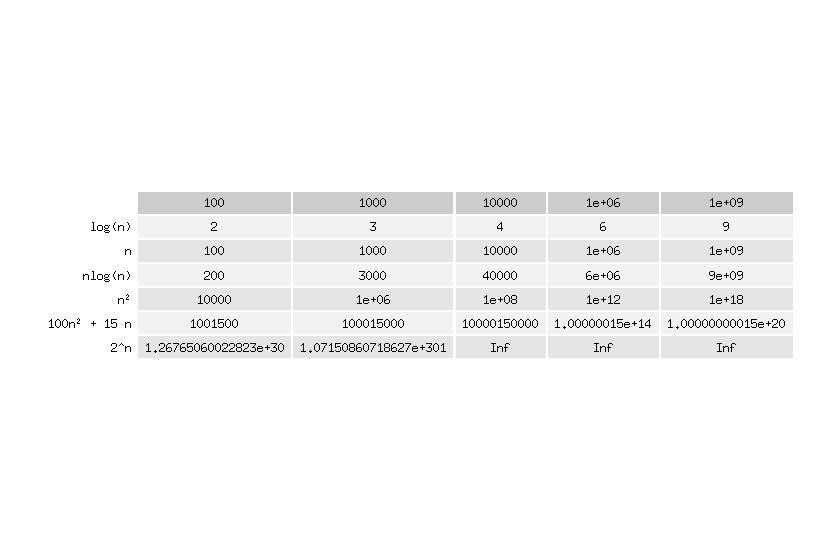
\includegraphics{Code/table_complexity}%


\end{document}